\chapter{Team 6 Agent Design}\label{team_6_agent_design}

\section{Overview}

In this chapter, we present the technical formulation and results of the Team 6 agent. This chapter is divided into seven parts and is structured as follows: 
\begin{enumerate}
    \item Specification of the agent structure (\Cref{agent-specification}).
    \item Introduction of the underlying concepts upon which the agent's behaviour is based (\Cref{social_motives}). 
    \item Demonstration of how the agents utilise common pool resources according to the concepts defined in the previous section (\Cref{food_consumption}). 
    \item Explanation of how a social network is formed through the concept of trust (\Cref{trust}).
    \item Exploration of how the agents communicate and interact with each other in order to self-organise (\Cref{self-organization}).
    \item Presentation and discussion of experimental results through simulations (\Cref{simulation_results}).
    \item Conclusion and future work (\Cref{conclusion_future_work}).
\end{enumerate}

Ultimately, we propose that this agent accurately parallels aspects of human nature through its capability to undergo behavioural change and formulate social connections with trust, and heavily and intelligently utilises treaties with an outlook to self-organisation.

%%%%%%%%%
%%%%%%%%% AGENT SPECIFICATION
%%%%%%%%%%%%%%%%%%%%%%%%%%%%%%%%%%%%%%%%%%%%%%%%%

\section{Specification of Agent Design}\label{agent-specification}

All agents \textit{i} $\in$ \textit{A} are implemented as a data structure, such that all agents contain sufficient parameterisation to participate in the various communication methods \textit{c} $\in$ \textit{C}, resulting in a set of interactions defined by I = $< \mathit{A, C} >$. Each agent inherits from the \textit{baseAgent} structure and also contains the fields contained in Table \ref{tab:agentStruct}. We note only the most relevant fields for quantifying the agent have been included.

\begin{table}[H]
  \begin{center}
    \begin{tabular}{c|c}
      \textbf{Parameter} & \textbf{Range}\\
      \hline
      \texttt{BaseBehaviour} & \textit{N} $\in$ [0,10]\\
     texttt{Stubbornness} & \textit{N} $\in$ [0,1]\\
      texttt{MaxBehaviourSwing} & \textit{N} $\in$ [0,10]\\
      texttt{ParamWeights} & \{ HPWeight:\textit{N}, FloorWeight:\textit{N} \} \\
      texttt{FloorDiscount} & \textit{N} $\in$ [0,1]\\
      texttt{MaxBehaviour} & \textit{N} = 10\\
      texttt{PrevFoodDiscount} & \textit{N} $\in$ [0,1]\\
      texttt{MaxTrust} & \textit{N} = 25\\
    \end{tabular}
    \caption{Parameters held in the \texttt{Config} data structure}
    \label{tab:agentConfig}
\end{center}   
\end{table}


\begin{table}[H]
  \begin{center}
    \begin{tabular}{c|c}
      \textbf{Parameter} & \textbf{Range}\\
      \hline
      texttt{BaseAgentRef} & texttt{*baseAgent}\\
      texttt{Config} & texttt{config}\{\} (see \Cref{tab:agentConfig})\\
      texttt{CurrBehaviour} & \textit{N}\\
      texttt{MaxFloorGuess} & \textit{N}\\
      texttt{AverageFoodIntake} & \textit{N}\\
      texttt{ShortTermMemory} & [\textit{N}]\\
      texttt{LongTermMemory} & [\textit{N}]\\
      texttt{ProposedTreaties} & [\textit{Treaty}] \\
      texttt{TrustTeams} & map\{ \textit{UUID}, \textit{N} \} \\
      texttt{Neighbours} & \{ above:\textit{UUID}, below:\textit{UUID} \} \\
    \end{tabular}
    \caption{Parameters held in the \texttt{Agent} data structure}
    \label{tab:agentStruct}
\end{center}   
\end{table}


%%%%%%%%%
%%%%%%%%% SOCIAL MOTIVES
%%%%%%%%%%%%%%%%%%%%%%%%%%%%%%%%%%%%%%%%%%%%%%%%%
\section{Social Motives}\label{social_motives}
%%
%% Theoretical Framework
%%
\subsection{Social Motives Spectrum}
The initial concept upon which this agent's behaviour is based revolves around the four possible social motives \cite{socMot} that this agent can have based on different principles, practices, or characteristics. This in turn leads to a ``mixed-motive'' setting \cite{schellingConflict} in the tower. These social motives are: 

\begin{itemize}
    \item \textbf{Altruism:} The disinterested and selfless concern for the well-being of others. An altruist then acts in a way that purely benefits others, even if it means harming themselves.
    \item \textbf{Collectivism:} The practice or principle of giving a group priority over each individual in it. A collectivist then acts in a way that benefits the group, themselves included, over purely the individual.
    \item \textbf{Selfishness:} Being concerned excessively or exclusively with oneself. A selfish agent will act in a way to satisfy themselves, but not necessarily with the intent to harm the other agents.
    \item \textbf{Narcissism:} An excessive interest or admiration of oneself. A narcissistic agent will act in a way that not only benefits themselves, but also hinders the collective.
\end{itemize}

For this implementation, we assert that all agents' social motives can be defined on a spectrum, with one end corresponding to pure altruism and the other end corresponding to pure narcissism. This is represented as a continuous value between 0.0 and 10.0 that shows where an agent lies in the social motive spectrum. Using a continuous rather than discrete variable for the social motive allows for greater expression: for example, two agents may both be referred to as collectivists, but one may be significantly closer to turning selfish than the other. A number closer to 0.0 corresponds to altruistic behaviour, and a number closer to 10.0 corresponds to narcissistic behaviour. The boundaries for the four distinct social motives are shown in Figure \ref{fig:socialMotives}. The initial “natural” state of a given agent and its current social motive are also shown and labelled \texttt{baseBehaviour} and \texttt{currentBehaviour}, respectively. To begin, we set \texttt{currentBehaviour} = \texttt{baseBehaviour}.

\begin{figure}[htb]
    \centering
    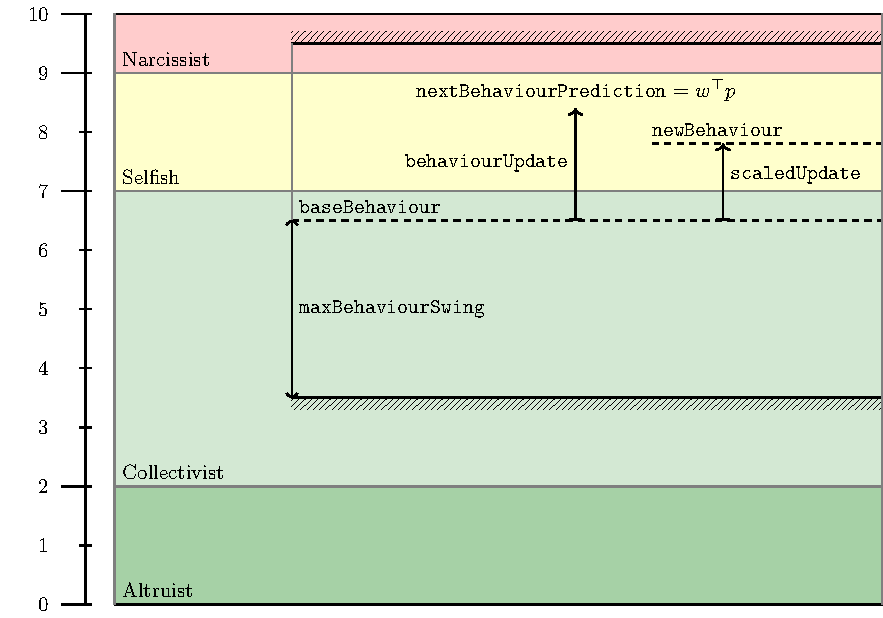
\includegraphics[width=0.9\textwidth]{008_team_6_agent_design/SOMAS_social_motives.pdf}
    \caption{Spectrum of social motives. An agent's behaviour is dependent on where it resides within this spectrum. Agents can also change throughout the game as signified by the arrows. Willingness to change is introduced to scale this behaviour update and bounds are placed to prevent extreme changes.}
    \label{fig:socialMotives}
\end{figure}


\subsection{Changing Social Motives}
Placing an agent into one of these fixed categories for the entire duration of the game would be limiting and unrealistic. This led to the addition of the first layer of complexity: given that an agent may be initially assigned a social motive, it should be plausible for the agent to change their social motive based on their experience. This concept brings forth the interesting duality of ``nature vs nurture'' \cite{natNur}. One could also think about this in terms of ``genotype vs phenotype''. For example, an agent may `naturally' or `genetically' be born a collectivist but may be incentivised to change its values and act selfishly if it becomes desperate due to a lack of food. In this environment, the factors that influence an agent’s social motive are its current HP and current floor, as both reflect an implicit lack of food.

The process of changing an agent’s social motive based on certain factors can be represented as a weighted sum of these factors. In this case, where the related parameters are the current HP value and the current floor, the weighted sum can be achieved by defining a parameters vector \textit{p} and a weights vector \textit{w}. The weighted sum is then given by the product $w^\top{}p$. These are shown below:


\begin{equation}
    \begin{gathered}
    p = [\mathit{currentHP, currentFloor}],\quad w=[\mathit{weightHP, weightFloor}] \\ 
    w^\top{}p = \mathit{weightHP \cdot currentHP + weightFloor \cdot currentFloor}
    \end{gathered}
\end{equation}



\subsubsection{Feature Transformations} \label{sec:featTran}

Instead of using the values of \texttt{currentHP} and \texttt{currentFloor} directly, we use transformation functions to map them into an output domain between 0 and 1. These transformations additionally allow us to associate a non-linear importance to a given factor. We refer to the resulting factors as \texttt{hpScore} and \texttt{floorScore} respectively.

The $hpScore$ is calculated as

\begin{equation}
    \mathit{hpScore} = 1 - \frac{\mathit{currentHP}}{\mathit{maxHP}}
\end{equation}

yielding a simple linear mapping (\texttt{HP} $\in$ [0,100] $\rightarrow$ [1,0]), where a higher \texttt{currentHP} maps to a lower \texttt{hpScore}, resulting in a tendency for the agent to behave more altruistically.

Calculating the \texttt{floorScore} requires knowledge of the maximum floor in the tower. As this information is not available to the agent, it will use its memory of the past floors it has been on to forecast this value. Furthermore, the mapping is non-linear, with lower floors (higher number) being `punished' more; how much more is determined by the parameter $\lambda$, where a greater $\lambda$ weights lower floors disproportionately more. This gives:

\begin{equation}
    \mathit{floorScore} = \frac{e^{\frac{\lambda\cdot \mathit{currentFloor}}{\mathit{maxFloor}}}}{e^{\lambda}}
\end{equation}

A lower floor (higher floor number) leads to a higher \texttt{floorScore} resulting in a tendency of the agent towards narcissism.

\subsubsection{Dynamic Weights}

This agent offers an additional level of complexity regarding the way it weights the utilities of both its current health and floor in the tower. We propose the idea that if an agent is consistently evaluating the utility of one of the aforementioned parameters as low, they should assign it a higher weighting so as to encourage a greater shift towards narcissistic behaviour for self-interested survival.

To achieve this, we update the behavioural weights as follows:

\begin{itemize}
    \item If the agent's health is less than 20:
    \begin{enumerate}
        \item \texttt{weightHP} $\leftarrow$ \texttt{weightHP} + 0.05
        \item \texttt{weightFloor} $\leftarrow$ \texttt{weightFloor} $-$ 0.05
    \end{enumerate}
    \item If the agent's average food intake is less than 1:
    \begin{enumerate}
        \item \texttt{weightHP} $\leftarrow$ \texttt{weightHP} $-$ 0.1
        \item \texttt{weightFloor} $\leftarrow$ \texttt{weightFloor} + 0.1
    \end{enumerate}
\end{itemize}

In addition, we use sufficient boundary conditions to ensure that the individual weights consistently fall within the range [0,1].

\subsubsection{Behavioural Update}

Based on the mapping of social motives from 0.0 to 10.0, a lower floor (i.e., greater floor number) and a lower HP push the social motive variable to be higher. The weights are hence chosen to reflect these correlations (initialised as 0.3 resp. 0.7), along with the relevant feature transformations (\Cref{sec:featTran}) applied to these factors.

This weighted sum represents the prediction of the agent's next social motive, titled \texttt{nextBehaviourPrediction} in \Cref{fig:socialMotives}. We therefore calculate:

\begin{equation}
    \mathit{behaviourUpdate = nextBehaviourPrediction - currentBehaviour}
\end{equation}


For the first iteration, \texttt{currentBehaviour} = \texttt{baseBehaviour} as presented in \Cref{fig:socialMotives}.

\subsection{Willingness to Change}
Although the above encapsulates an essential human characteristic, the ability to change, another important element, the willingness to change, is missing. Through this next layer of complexity, we attempt to quantify how resistant an agent is to altering its behaviour. This concept brings forth more freedom for modelling different human characteristics and realistic situations. For example, it is now possible to distinguish between an agent that is initially an altruist, but may then become selfish as the supply of food diminishes, and an agent that is a “true altruist”, which retains the same social motive throughout. Similarly, this is extended to the distinction between a true narcissist agent that never changes, and a narcissist agent that may, during the game, witness others' suffering whilst itself has an abundance of food and therefore steer towards a more collectivist behaviour.

To represent the willingness of an agent to change its social motive, an additional parameter, labelled as \texttt{stubbornness}, is introduced and instantiated as a number between 0.0 and 1.0. This number is used to scale the behaviour update. This operation is similar to a step-size, and reflects how easy it is for the social motive to change. We therefore calculate the \texttt{scaledUpdate} and \texttt{newBehaviour} as shown below.


\begin{equation}
    \begin{gathered}
    \mathit{scaledUpdate = behaviourUpdate \cdot (1-stubbornness)} \\
    \mathit{newBehaviour = currentBehaviour + scaledUpdate}
    \end{gathered}
\end{equation}


Again, \texttt{currentBehaviour} = \texttt{baseBehaviour} for the first iteration.

\subsection{Bounding Change}
The agent we propose is currently assigned an initial social motive and is then able to change throughout the duration of the game. The ease with which it changes is also quantified through its willingness to change. This brought forth the possibility that even though an agent might be stubborn/resistant to change, it is still, given a long enough period, able to go from a narcissist to an altruist. This, considered to be unrealistic, lead to the final addition of complexity concerning the prevention of extreme changes in social motive. Prior to the start of the game, we define how far an agent can steer away from their `genetic' or `natural' initial state.

Bounding social motive change is modelled through the addition of the parameter \texttt{maxBehaviourSwing}. This parameter allows for the definition of the maximum and minimum values of the allowed social motive for an agent, thus defining a range:

\vspace{0.2cm}
\begin{equation}
    \begin{gathered}
    \mathit{max = baseBehaviour + maxBehaviourSwing}  \\
    \mathit{min = baseBehaviour - maxBehaviourSwing}
    \end{gathered}
\end{equation}
\vspace{0.2cm}

If the change as defined in Step 3 results in a \texttt{newBehaviour} outside this range, then this is automatically capped off at the edges. Naturally, this also holds for the spectrum edges $[0,10]$.



% %%
% %% Mathematical Formulation
% %%
% \subsection{Mathematical Formulation}\label{mathematical_formulation}
% In order to implement this agent’s behaviour, we present a mathematical formulation and its implementation for each of the steps introduced above.

% \subsubsection{Define Social Motives}



% \subsubsection{Changing Social Motives}



% \subsubsection{Willingness to Change}


%%%%%%%%%%
%%%%%%%%%% FOOD COMSUMPTION
%%%%%%%%%%%%%%%%%%%%%%%%%%%%%%%%%%%%%%%%%%%%%%%%%%%%%%
\section{Food Consumption}\label{food_consumption}
%%
%% Strategy
%%

% \subsection{Conceptual Description}
\subsection{Variation by Social Motive}
With the agent's behavioural theory defined, its corresponding strategy can be expressed based on the defining qualities of its social motive. As the social motive varies from Altruist towards Narcissist, individual utility is valued increasingly more than collective utility, resulting in an increase in food consumption. Whilst social motives are defined using a continuous spectrum, the agent’s consumption and communication strategies are defined on bins along this spectrum, with one bin for each of the four discrete social motives. Thus, which strategy is carried out is decided in a switch-case statement on the agent's current behaviour.


% \subsubsection{Altruist}
% Since an altruistic agent is only concerned for the well-being of others with total disregard for itself, it takes no food and aims to maximise the amount of food left for the remaining agents.

% \subsubsection{Collectivist}
% A collectivist will consume the minimum food needed to survive. The result is that, on injection, this agent takes no food due to having high starting health. As turns progress, when the agent approaches a critical condition, it takes the minimal amount to satisfice itself. Since there is a time delay between when this agent first falls critical and is terminated, we assert that all collectivists stagger the day that they take food (randomised between 1 and the maximum number of days an agent can stay critical for) to ensure that all the available resources are not depleted at one given time.

% \subsubsection{Selfish}
% A selfish agent will consume enough food to be satiated and remain `healthy'. In this report, we define satiation to represent a health of at least 30\% of the maximum value.

% \subsubsection{Narcissistic}
% A narcissistic agent will consume the maximum amount of food possible to take at a given iteration, since it will purely be concerned for its well-being and be willing to harm other agents.


\subsubsection{Altruist}
An altruistic agent will always take 0 food, as it is only concerned for the well-being of others with a total disregard for itself.

\subsubsection{Collectivist}
A collectivist agent will consume just enough food to survive, and consume no food when not in danger of dying. Based on the implemented health function, the agent is only in danger of dying when in the Critical region, and will die if it spends \texttt{N = maxCritical} days in this zone without consuming the minimum required units of food to return to the \texttt{WeakLevel}. The collectivist agent, having entered the Critical region, will consume food on a randomly assigned day within the allowable period to leave the Critical region. The day of consumption is randomised to avoid the case of all agents needing to consume food on the same day, as there is not enough food on the platform to satisfice every agent in the tower at one time.

% \begin{verbatim}
% case "Collectivist": // Only eat when in critical zone randomly before expiry
%     switch {
%     case currentHP >= levels.weakLevel:
%         a.foodTakeDay = rand.Intn(healthInfo.MaxDayCritical) // Stagger eating days
% 	    return food.FoodType(0)
%     case currentHP >= levels.critLevel:
%         if a.DaysAtCritical() == a.foodTakeDay {
%             return food.FoodType(healthInfo.HPReqCToW)
%         }
%         return food.FoodType(0)
%     default:
%         return food.FoodType(0)
%     }
% \end{verbatim}

\begin{itemize}
    \item If this agent has health $\geq$ \texttt{weakLevel}:
    \begin{enumerate}
        \item Assign \texttt{allowedFoodTakeDay} to \texttt{rand(0, maxDaysCritical)}
        \item Take 0 food
    \end{enumerate}
    \item Else if this agent has health $\geq$ \texttt{criticalLevel}:
    \begin{itemize}
        \item If \texttt{allowedFoodTakeDay} matches the number of days that this agent has stayed critical: take 2 food
        \item Otherwise: take 0 food
    \end{itemize}
    \item Default: take 0 food
\end{itemize}

\subsubsection{Selfish}

A selfish agent consumes the amount of food required to remain in a healthy state. A healthy state is arbitrarily defined as between 30\% and 60\% of the maximum possible health. These values are assigned to variables \texttt{healthyLevel} and \texttt{strongLevel}, respectively, with the selfish agent operating accordingly under these three conditions:

\begin{itemize}
    \item If the agent's health is greater than or equal to the \texttt{strongLevel}: take 0 food
    \item If the agent's health is between \texttt{healthyLevel} and \texttt{strongLevel}: take enough food to maintain the current HP value
    \item If the agent's health is less than the \texttt{healthyLevel}, the agent takes enough food to reach the \texttt{healthyLevel}.
\end{itemize}


% Based on the health functions, the change in HP is formulated in equation \eqref{HP+}:

% \begin{equation}
%     HP = HP + w(1 - e^{\frac{x}{\tau}}) - b + s(\mathit{HP} - \mathit{weakLevel}) \label{HP+}
% \end{equation}

% $HP$ is the agent's current HP, $HP^+$ is the updated HP after consuming $x$ units of food. $b$ and $s$ are the base HP loss and the HP loss slope, defined in the health loss function, respectively. $w$ is the maximum possible HP gain. $\tau$ is the food required for the HP to increase by $0.63w$.

% Rearranging equation \eqref{HP+} to solve for food consumed $x$, the food required to reach some goal HP from the agent's current HP is formulated in equation \eqref{x_goal}:

% \begin{equation}
%     \mathit{x_{goal}} = \tau ln(w) - \tau ln(w - \mathit{HP_{goal}} + (1 - s)\mathit{HP} - b + s \cdot \mathit{weakLevel}) \label{x_goal}
% \end{equation}

% The above equation is implemented in a function that takes \textit{currentHP}, \textit{goalHP}, and \textit{healthInfo} as arguments and returns a \textit{food.FoodType} value in the following manner:
% \\
% BULLET POINTS
% \\
% \begin{equation}
%     \mathit{denominator} = 
% \end{equation}
% % \begin{verbatim}
% % func (a *CustomAgent6) foodRequired(goalHP float64, healthInfo *health.HealthInfo) food.FoodType {
% %     denom := healthInfo.Width - goalHP + (1-healthInfo.HPLossSlope)*a.HP()
% %             - float64(healthInfo.HPLossBase) 
% %             + healthInfo.HPLossSlope*float64(healthInfo.WeakLevel)
% %     return food.FoodType(healthInfo.Tau * math.Log(healthInfo.Width/denom))
% % }
% % \end{verbatim}

% This function is sufficient to implement the three conditions of a selfish agent. The selfish agent's strategy is implemented in the following case statement:
% \\
% BULLET POINTS
% \\
% % \begin{verbatim}
% %     case "Selfish": // Stay in Healthy zone
% %     switch {
% %         case currentHP >= levels.strongLevel:
% %             return food.FoodType(0)
% %         case currentHP >= levels.healthyLevel:
% %             return a.foodRequired(currentHP, healthInfo)
% %         default:
% %             return a.foodRequired(levels.healthyLevel, healthInfo
% %     }
% % \end{verbatim}

\subsubsection{Narcissist}

A narcissistic agent will take maximum amount of food consumable, since it is purely be concerned for its own well-being, to the chagrin of other agents.

% \begin{verbatim}
%     case "Narcissist": // Eat max intake
%         return healthInfo.maxIntake
% \end{verbatim}

%%
%% Implementation
%%
\subsection{Final Implementation}
The actual amount of food consumed by the agents in the final implementation does not solely depend on the social motives and the current health level, but also on other factors, such as trust, and commitments on messages and treaties. The dependency on these other factors will be explored in the corresponding sections.


%%%%%%%%%%
%%%%%%%%%% TRUST
%%%%%%%%%%%%%%%%%%%%%%%%%%%%%%%%%%%%%%%%%%%%%%%%%%%%%%
\section{Formation of Social Network through Trust}\label{trust}

\subsection{Background}

With treaties offering a notion of socially accepted institutional power, the formation of treaties must be handled carefully so as not to disadvantage the agents who engage in them. For this reason, a social network must be constructed to offer a heuristic for joining into these agreements. 

Trust serves as ``an important role for the formation of coalitions in social networks and in determining how high value of information flows through the network'' \cite{trustEEE}, with Ostrom further supporting that ``trust is an essential social lubricant'' \cite{ostrom2003trust}. Ostrom further asserts that trust ``affects the willingness to cooperate'' \cite{ostrom2003trust} and ``enhances cooperation in social-dilemma experiments'' \cite{ostrom2003trust}, providing clear reasoning that trust is an effective parameter to introduce to the agent structure.

Finally, it is through this introduction of trust that we demonstrate the assertion from Adali's work \cite{trustEEE} that trust facilitates ``communication behaviors which are statistically different from random communications''.

\subsection{Initialisation}
The agent takes a simple algorithmic approach to formulating a social network: first, the ID of the neighbouring agents is determined through message passing; this ID is mapped to an initial trust value which is continually updated through subsequent social interactions. 

This agent implementation offers different initialised trust values based on the social motive, using the general notion that the more narcissistic an agent is, the less likely it is to have an initial positive opinion of their neighbours. 

For this reason, we give a maximal range of trust from $-25$ to +25 with the initialisations as follows:
\begin{itemize}
    \item Narcissist: $-5$
    \item Selfish: 0
    \item Collectivist: +5
    \item Altruist: +10
\end{itemize}

\subsection{Causes for Trust Update}

It is through continuous social interaction in the tower that agents will be able to form opinions of the other agents. For this agent, there is a specific set of interactions that will result in a opportunity for trust to update. These interactions impose a \textit{base} behavioural update, before scaling due to social motive (\Cref{sec:varTrust}).

\subsubsection{Treaties}

\begin{enumerate}
    \item When an agent receives a response to the treaty it has proposed: 
    \begin{itemize}
        \item If accepted: +3
        \item If rejected: $-2$
    \end{itemize}
    \item When an agent receives a treaty proposal: 
    \begin{itemize}
        \item  If the treaty is evaluated as good: +2
        \item   If the treaty is evaluated as bad: $-1$
    \end{itemize}
\end{enumerate}

\subsubsection{Communications}

\begin{enumerate}
    \item If an agent makes a request for another to take 0 food (\Cref{sec:takeNone}):
    \begin{itemize}
        \item  If accepted: reset to 0
        \item  If rejected: $-1$
    \end{itemize}
    \item If an agent is requested to leave food: 
    \begin{itemize}
        \item If narcissist: $-1$
        \item Otherwise: +0
    \end{itemize}
    \item If an agent is requested to take a certain amount of food: $-1$
\end{enumerate}

\subsubsection{Case of Low Trust} \label{sec:takeNone}

If an agent holds an extremely low opinion of another agent (trust $\leq -10$), it will send a message asking the other to take 0 food for one turn, so as to restore trust and show repentance. If this agent accepts the request, it is forgiven and has its trust value reset to 0. If not, the opinion of this agent is decremented.

\subsubsection{Case of Low Average Food} \label{sec:lowFood}

If an agent continually averages less than one unit of food per day, it makes the assumption that the agent above is acting maliciously. For this reason, the trust of this neighbouring agent is decremented. Conversely, if the agent is averaging above this amount, it will increment its trust in the neighbour above.

\subsection{Variations in Trust Update} \label{sec:varTrust}

To maintain a strong sense of social cohesion, the trust assigned to another agent must be continually updated to reflect the ongoing exchange of information \cite{trustEEE}. Again, this agent implementation asserts that the different social motives will have different responses to positive and negative interactions, with the magnitude of the change in trust varying proportionally. This scaling is documented below.

In the case of a positive exchange, the scaling is as follows:
\begin{itemize}
    \item Narcissist: $\times 0$
    \item Selfish: $\times 1$
    \item Collectivist: $\times 2$
    \item Altruist: $\times 4$
\end{itemize}

If the agent is currently acting as a narcissist it is impossible to increase its opinion of another agent. This agent must undergo considerable environmental change to update its behaviour towards the altruistic side of the spectrum to increase trust.

Conversely, in the case of a negative exchange, the trust of another agent will \textit{decrease} as follows:
\begin{itemize}
    \item Narcissist: $\times 4$
    \item Selfish: $\times 2$
    \item Collectivist: $\times 1$
    \item Altruist: $\times 0$
\end{itemize}


%%%%%%%%%%%
%%%%%%%%%%% SELF-ORGANIZATION
%%%%%%%%%%%
\section{Approach to Treaties}\label{self-organization}

Messages allow for short-lived communication between two neighbours. With request and response messages, such as “leave X food on the platform”, agents can organise locally. However, to establish a stable, self-organising system across many floors and many reassignment periods, a more sophisticated form of agreement is necessary. For this reason, an agent's strategies rely heavily on treaties, mimicking research findings from the field of behavioural psychology.

To successfully handle treaties, an agent must:
\begin{enumerate}
    \item Rate treaties
    \item Change its behaviour based on accepted treaties
    \item Propose treaties
\end{enumerate}


\subsection{Types of Treaties}

As food is a scarce resource in the tower, the main purpose of self-organisation should be to limit how much food agents eat. By handling all possible conditions, (``less than'', ``less than or equal'', ``equal to'', ``greater than or equal to'', ``greater than''), this strategy focuses on assigning upper bounds to the amount of food eaten.

To ensure that an agent has access to food on a given turn, it is integral for the neighbouring agents to \texttt{leave} food, wherein the infrastructure of the tower provides multiple types of treaties: \texttt{LeaveAmountFood}, \texttt{LeavePercentageFood} and \texttt{Inform}. To enforce localised sanctions and suggest an intake of food to allow stability, however, what really counts is the amount of food taken. Thinking in terms of the \texttt{LeaveFood} types limits how much treaties can distribute through the tower: \texttt{LeaveAmountFood} would allow the first few agent floors to eat as much as desired without breaking the treaty. Once this amount is reached, any subsequent agent does not receive anything. Similarly, \texttt{LeavePercentageFood} limits agents by exponentially decreasing portions, such that low levels have little chance of surviving even if everyone satisfies the treaty. \texttt{TakeAmountFood} does not face this issue as it limits consumption no matter the amount of food an agent has access to. Consequently, the agent thinks in terms of the amount food it takes, converting any other treaty type to an equivalent upper bound of food it is allowed take. This makes it easier to compare treaties and make sure that accepted treaties are not contradicting one another.

Having clarified the general interpretation of treaties, we now describe the two main underlying principles with which we handle treaties: Forecasting and Utility Theory.

\subsection{Forecasting for Resource Availability} \label{sec:forecasting}

\subsubsection{Theory}

Treaties do not have any immediate effect, but instead influence the future consumption of an agent. In order to assess the present value of a treaty, an agent greatly benefits from the ability to predict its future.

In the case of this tower, ``future'' can mean two different things: the future of an agent on the current level and their future on a series of unpredictable levels after that. An example of this may be that an agent very high up in the tower can expect to receive a surplus of food in the coming days, but should not expect the same in future reshuffling periods. The future on this floor is best predicted by the previous experience on this floor, while the future thereafter is best predicted by all previous experience in the tower. Accordingly, we assert that each agent separately keeps track of the amount of food it receives each day during the current reassignment period as well as through its entire lifetime. This aligns well with the core assumption in cognitive psychology that there are separate systems for long- and short-term memory \cite{norris2017short}.

\subsubsection{Implementation}
To implement forecasting, we use two separate arrays corresponding to long-term and short-term memory and store the amount of food received each day (\Cref{fig:forecasting}).

The short-term memory is reset after every reshuffle and a scaled histogram illustrating the number of times the agent has received a certain amount of food results in a discrete distribution that can be used for predicting the expected food in the future.

\begin{figure} [htb]
    \centering
    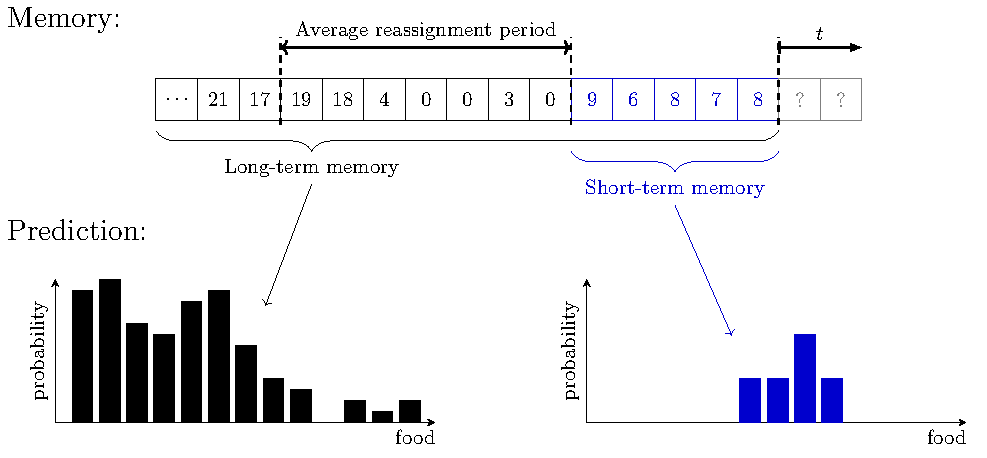
\includegraphics[width=0.9\linewidth]{008_team_6_agent_design/SOMAS_forecasting.pdf}
    \caption{Forecasting of the estimated food received in the short-term and long-term using two integer arrays.}
    \label{fig:forecasting}
\end{figure}

In order to distinguish between the short and long term, this agent also forecasts how long it will stay on the current floor. It does so by averaging the duration of previous reshuffling periods.

\subsection{Utility Theory}

Memory allows an agent to remember the past; forecasting uses this to predict the future. In order to make a decision regarding treaties, one last step is required: the agent needs to be able to compare two potential futures and decide which one it deems more beneficial.

Behavioural research has shown that the satisfaction of gaining or losing wealth is non-linear \cite{fishburn1988nonlinear} and utility functions are commonly used to account for this by mapping the monetary value of a good or service to an individual's preference \cite{fishburn1970utility}. To accurately model human decision making, this agent uses utility functions to make decisions regarding food as the one scarce good in the tower.

We program this agent to use utility functions as a mechanism to compare which of two different futures is more beneficial. To achieve this, the agent calculates the expected utility both with and without a treaty, subsequently maximising its estimated future benefit by choosing the larger expected utility. The expected utility from gaining a certain amount of food $a$ is deterministic, hence:

\begin{equation}
    E[U(a)] = U(a) 
\end{equation}

The utility of gaining an uncertain amount of food represented by the discrete random variable $x$ (based on past experience), is computed with:

\begin{equation} 
x = [ p_1: x_1, p_2: x_2; ... \;p_n: x_n]
\end{equation}

where an agent expects to get amount $x_i$ of food with probability $p_i$, such that

\begin{equation}
E[U(x)] = p_1 \times U(x_1) + p_2 \times U(x_2) + ... + p_n \times U(x_n)
\label{eq:expectedUtility}
\end{equation}

\subsubsection{Prospect Theory}

Comparing potential future outcomes with utility allows for the introduction of known psychological behaviours to the agents. Prospect theory, first established by Kahneman and Tversky \cite{kahneman2013prospect}, is a well-established model of how a change in value is perceived or, alternatively, how much utility is gained or lost from a change in value (\Cref{fig:prospect}). 

\begin{figure} [htb]
    \centering
    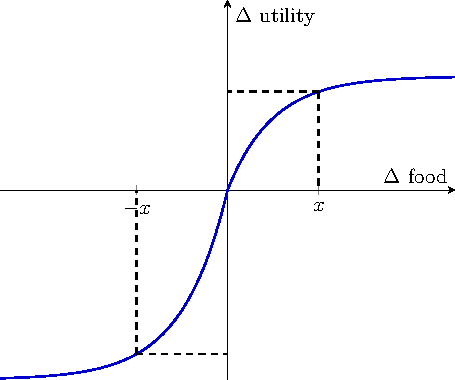
\includegraphics[width=0.5\linewidth]{008_team_6_agent_design/SOMAS_prospect_theory.pdf}
    \caption{Utility in decision making according to prospect theory.}
    \label{fig:prospect}
\end{figure}

This model comprises three main principles:
\begin{itemize}
    \item \textbf{Greediness:} Humans are generally greedy, meaning that more of something is always at least regarded as beneficial. Utility functions are hence generally increasing.
    
    \item \textbf{Diminishing sensitivity:} Marginal returns are strictly decreasing, thus, the greater the personal wealth of an agent, the less they value the resource. An additional unit of food matters much more to an agent if it only gets one unit of food compared to if it gets 50 units of food.
    
    \item \textbf{Risk aversion:} Humans generally try to avoid risk. The discrete random distribution which forecasts the expected food received does not guarantee any certain amount of food and so is associated with risk. With risk aversion, the amount of food the agent perceives as equivalent to a random distribution, its \textit{certainty equivalent} $C$, is hence less than its mean.

    \begin{equation}
    U(C) = E[U(x)] < U(E[x])    
    \end{equation}
    
    \item \textbf{Loss aversion:} Losing some amount of food is generally perceived as worse than gaining that same amount. To account for this, the agents weigh losing an amount of food stronger than gaining the same amount of food.
\end{itemize}

\subsection{Social Motives and Total Utility}

Prospect theory forms the basis to how the agents' benefit from a change in consumption is modelled. In addition to the \textit{gain}, however, there is also a \textit{cost} that increases with eating more food: every unit of food gained is one unit of food other agents lose. This social cost, combined with the previously explained explained utility, forms the total utility function of \textit{x}, the amount of food received, given by 

\begin{equation}
    U(x)=gx^\frac{1}{r}-cx.
\end{equation}

Each of the social motives correspond to different values of greediness, risk-aversion, and social cost, which have been chosen according to three insights: 
\begin{enumerate}
    \item The more selfish an agent is, the greedier it is.
    
    \item The more an agent cares for the greater good, the greater its social cost associated with consumption.
    
    \item Studies have shown that more narcissistic people are generally less risk-averse \cite{campbell2004narcissism}.
\end{enumerate}

We choose the parameters for each social motive accordingly, with greediness $g$, risk-seeking $r$ and social responsibility $c$, resulting in the total utility functions in \Cref{fig:utilities}.
\begin{enumerate}[label=(\alph*)]
    \item \textbf{Altruist}: not greedy, very risk-averse, very high social responsibility
    
    \item \textbf{Collectivist}: slightly greedy, risk-averse, high social responsibility
    
    \item \textbf{Selfish}: greedy, low risk-aversion, low social responsibility
    
    \item \textbf{Narcissist}: very greedy, very low risk-aversion, no social cost
\end{enumerate}

\begin{figure}[htb]
    \centering
    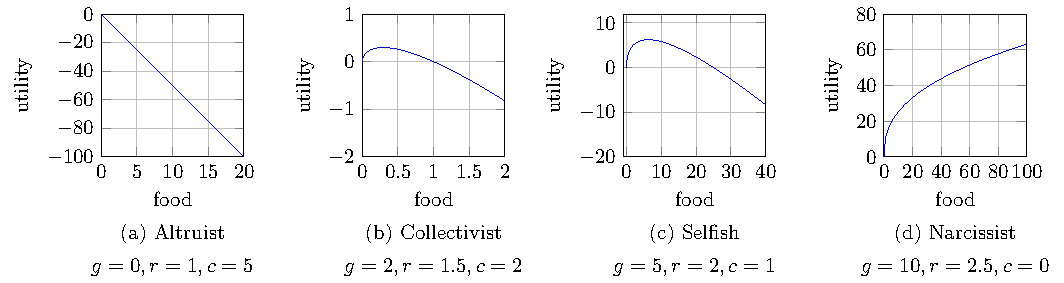
\includegraphics[width=0.95\linewidth]{008_team_6_agent_design/utility_functions/utility_functions.pdf}
    \caption{Different utility functions used to rate treaties according to the social motive of the agents. The associated parameters $g,r,c$ fully define the shapes of each utility function.}
    \label{fig:utilities}
\end{figure}


\subsection{Short and Long Term Trade-Off}

As mentioned in \Cref{sec:forecasting}, the futures the agent should expect in the short (on the current level) and long term (throughout the tower) differ. The longer the duration of a treaty, the more the long-term benefit should matter. By using the short and long term memory of food received each day, the agent can separately estimate the resources it can expect to gain on the current floor and how much it can expect to gain (on average) across all future reassignment periods.

By calculating the length of the average reassignment period, the agents can estimate the number of days remaining on the current floor. We use the proportion of estimated days before the next reshuffling period to the duration of the treaty in order to weigh how much an agent should focus on the short term. Let $b_\text{short}$ and $b_\text{long}$ be the estimated long and short term benefit of a treaty, respectively. Also, let the estimated days remaining on the current level be given by $d_\text{current}$ and the duration of a treaty by $d_\text{treaty}$. The total benefit $b_\text{tot}$ is given by

\begin{equation}
b_\text{tot} = d\times b_\text{short} + (1-d)\times b_\text{long}    
\label{eq:shortlongweight}
\end{equation}

where $d = \frac{d_\text{current}}{d_\text{treaty}}$.

The following examples show how this plays out.

\begin{itemize}
    \item $d_\text{current} = 10$, $d_\text{treaty} = 8\Rightarrow d=100\%$ (treaty expires before leaving the current floor)
    \item $d_\text{current} = 10$, $d_\text{treaty} = 20\Rightarrow d=50\%$
    \item $d_\text{current} = 10$, $d_\text{treaty} = 100\Rightarrow d = 10\%$
\end{itemize}


\subsubsection{Survival Instinct}

When one is doing well, the above weighting between the long and short term benefits is sensible. However, if one is struggling to stay alive, survival instincts kick in. Consequently, the agents ignore the expected long-term utility all together when their health is on a critical level.

\subsection{Implementation}

How agents rate treaties closely follows the theoretical steps from above. Every day, the agent stores the amount of food received in two arrays, one for the short and one for the long term. The short-term array is reset after every reshuffling period. When a new treaty is proposed, the agent performs the following steps to conclude whether to sign this new treaty or not:
\begin{enumerate}
    \item Check if the trust in the proposer agent is high enough.
    \item Check if the treaty is compatible with treaties that the agent signed already.
    \item Calculate the expected short- and long-term utility using the memory of food received in the past according to \Cref{eq:expectedUtility}. The utility function used depends on their current social motive.
    \item Amplify the utility if it is negative in accordance with loss-aversion.
    \item Estimate the amount of food it can take under the treaty, i.e., the difference between the average amount of food it received in the past and the amount of food it needs to leave in order to comply with the treaty, and calculate the utility of taking that amount of food.
    \item Compute the estimated short-term and long-term benefit of signing the treaty as $U(\text{sign}) - U(\text{don’t sign})$.
    \item Choose whether to focus on the long-term or short-term benefit according to \Cref{eq:shortlongweight}.
    \item Sign the treaty if its overall benefit is positive.
\end{enumerate}

The amount of food that the “collectivist” and “selfish” agents would need to consume in order to maximise utility varies depending on the current health level. The peak of its total utility function thus needs to be able to vary as well. We account for this by introducing a scaling factor $a$ as

\begin{equation}
    U(x)=g(ax)^\frac{1}{r}-cax
\end{equation}

where

\begin{equation}
    a=\frac{1}{z}\left(\frac{cr}{g}\right)^\frac{r}{1-r}
\end{equation}

introducing the desired food intake $z$ as the maximum of the function without changing the general properties of the function, leading to:

\begin{equation}
U\left(x\right)=g\left(\frac{1}{z}\left(\frac{cr}{g}\right)^{\frac{r}{1-r}}x\right)^{\frac{1}{r}}-cx\frac{1}{z}\left(\frac{cr}{g}\right)^{\frac{r}{1-r}}    
\end{equation}
\subsection{Behaving According to Treaties}

Treaties are fundamentally built on the assumption that all agents behave truthfully. Introducing dishonesty to treaties would sap them of all their power, as there are too many possible falsities but no sufficient way of recognising them and no central authority to punish them. Hence, we do not consider deception. Since this means that an agent cannot act against any active treaties, the amount of food taken has to be chosen with care.

We implemented a function to return the valid range of possible food intakes given a list of active treaties and accepted request messages, and use this both to check if a newly proposed treaty is compatible with previously accepted treaties and to \textit{legally} take food. We do this as in Algorithm \ref{code:treatyRange}.
% \Cref does not seem to work with algorithm components

 \begin{algorithm}
        \SetKwInOut{Input}{Input}
        \SetKwInOut{Output}{Output}
        \Input{List of active treaties \textbf{$T$}, RequestLeaveFood message \textbf{$M$}}
        \Output{Maximum amount of food allowed: \textbf{max}}
        \BlankLine
        max $\gets$ food received \
        \BlankLine
        \ForEach{$t \in T$}
        {
        \uIf{\textup{agent state} $\in$ $t$ \textup{condition}}{
            takeAmount $\gets$ convert $t$ request value
            
            \uIf{\textup{takeAmount} $\leq$ \textup{max}}{
                max $\gets$ takeAmount
            }

        }
        \BlankLine
        \uIf{\textup{neighbour requested to leave food}}{
            takeAmount $\gets$ convert $t$ request value
            
            \uIf{\textup{takeAmount} $\leq$ \textup{max}}{
                max $\gets$ takeAmount
            }
        }            
        }
        \caption{Function to ensure that an agent never breaks any accepted treaties.}
        \label{code:treatyRange}
\end{algorithm}

An agent then consumes the amount less than or equal to the resulting upper-bound \textit{max} that maximises their utility.


\subsection{Proposing Treaties}\label{proposing_treaties}


Treaty proposals are fundamentally linked to each agent's social motive, given that they work to the benefit of collective utility. The terms of each treaty must be adhered to by both entities that have agreed to it, resulting in a situation where both agents will benefit the same amount. Aligning this with agent strategies, a true narcissistic agent, which would go so far as to behave with the intention of causing detriment to others, would not make any decisions that might benefit its neighbouring agents. As a result of this, the narcissistic agent would not propose any treaties, as even though it might reap the rewards of a treaty, it will never offer other agents any assistance. On the other end of the spectrum, an altruistic agent that always makes decisions based on maximising other agents' utility, would not behave in a way that might benefit itself. This too has the effect of an altruist never proposing any treaties, as although it might offer aid to other agents, this would go against its self-sacrificing nature.

The collectivist and selfish agents are therefore the two social motives that propose treaties. The collectivist agent wishes to maximise collective utility by forming agreements that will increase the chances of itself and its neighbours surviving and the selfish agent wishes to maximise its own survival chances as it knows that agreeing to a treaty will bring personal benefits.

The possible treaties that could be proposed are set based on the different social motives. These were changed for testing purposes (see \Cref{simulation_results}), however, the basic structure is outlined below:
\begin{itemize}
    \item Collectivist: If the agent's health is above the \texttt{weakLevel}, leave 100\% of resources on the platform
    \item Selfish: If the agent's health is above the \texttt{strongLevel}, leave 100\% of resources on the platform
\end{itemize}

\subsubsection{Propagating Treaties}

Once a treaty has been accepted or rejected by an agent, it is possible for that agent to propose the same treaty to their neighbour. For a given agent, the main motivation behind propagating a treaty is to further increase the benefits of that treaty for that agent. Depending on the agent's social motive, the treaty might benefit their individual utility, the collective utility, or both. Following similar principles used for treaty proposals, we assert that all agents other than narcissists would be active in propagating treaties.

The altruist agent, though it may not accept the treaty, will still propagate it in order to maximise the utility of other agents. The collectivist agent will propagate treaties which it has itself accepted, in the hope that it will further benefit collective utility. Finally, the selfish agent will propagate treaties with the aim of reaping the rewards of multiple treaties to benefit itself. As mentioned, the narcissist will not propagate any treaties as it acts to hinder existing collective utility and destroy other agents. 



%%%%%%%
%%%%%%% SIMULATION RESULTS
%%%%%%%
\section{Simulation Results and Discussion}\label{simulation_results}

%%
%% Hypothesis
%%
\subsection{Hypothesis}\label{hypothesis}
Before presenting the simulation results, we offer the following hypotheses we wish to verify. Given the aforementioned modeling approach, the following affirmations are hypothesised:
\begin{enumerate}

    \item In a purely narcissist system, it is impossible for an agent to survive on a long-term basis.
    
    \item In a purely collectivist system, a stable state is reached.
    
    \item In a system composed of agents with different social motives, a polystable, i.e., a system that has more than one convergent state, ``whose parts have many equilibria'' \cite{ashby2015design}, can be reached in a long-term scenario.
        
    \item There exists a threshold on the number of selfish agents that can be incorporated in the system before a stable collectivist system becomes unstable.
     
    \item In a system composed of agents with different social motives, the ability to self-organise through treaties improves the global utility.
    
    \item In a system composed of agents with different social motives, where genetic replacement of the agents occurs, the system converges to a collectivist system.
   
   
\end{enumerate}

%%
%% Summary of simulation
%%
\subsection{Summary of Simulations}\label{simulation_summary}

To examine the different hypotheses introduced in \Cref{hypothesis}, different simulations need to be executed. We divide the simulations into five groups characterised by having different initialisation parameters. \Cref{tab:simulation_summary_1} and \Cref{tab:simulation_summary_2} summarise the simulation parameters. The percentages of each social motive correspond to the initial distribution. If not explicitly mentioned, we run experiments using 100 agents, with 100 food on the platform for 60 days and with a reshuffle period of 30 days. We also impose that this is a homogeneous tower, implementing only agents of this type (Team 6).

\begin{table}[h]
\centering
\begin{tabular}{l|llllllll}
                  & A1  & A2 & A3 & A4 & B1  & B2  \\ \hline
\% Altruist       & 100 & 0  & 0  & 0  & 10  & 5    \\
\% Collectivist   & 0   & 100& 0  & 0  & 40  & 60   \\
\% Selfish        & 0   & 0  & 100& 0  & 40  & 30   \\
\% Narcissist     & 0   & 0  & 0  & 100& 10  & 5    \\
Stubbornness      & -   & -  & -  & -  &  -  & -    \\
MaxBehaviourSwing & 0   & 0  & 0  & 0  &  0  & 0    \\
Communication     &yes  & yes&yes &yes & yes & yes
\end{tabular}
\caption{Summary of the experiments A1 to B2. The agents are not able to change their social motives.}
\label{tab:simulation_summary_1}
\end{table}

\begin{table}[h]
\centering
\begin{tabular}{l|llllllll}
                  & C1 & C2 & C3 & D1  & D2 & E1 & E2 \\ \hline
\% Altruist       & 10 & 10 & 10 & 100 & 100& 25  & 25 \\
\% Collectivist   & 40 & 40 & 40 & 0   & 0  & 25  & 25 \\
\% Selfish        & 40 & 40 & 40 & 0   & 0  & 25  & 25 \\
\% Narcissist     & 10 & 10 & 10 & 0   & 0  & 25  & 25 \\
Stubbornness      & 0.2& 0.2& 0.2& 0.8 & 0.8& 0.2 & 0.2\\
MaxBehaviourSwing & 8  & 8  & 8  & 6   & 6  & 6   & 2 \\
Communication     & yes&no  &yes & yes &yes & yes & yes
\end{tabular}
\caption{Summary of the experiments C1 to E2. The agents are able to change their social motives.}
\label{tab:simulation_summary_2}
\end{table}

In addition, cases C3, D2, E1 and E2 have additional specific features. In comparison to C1, C3 introduces more restrictive treaties. This is also the case for D2. In simulation E1 and E2, we use a a concept approaching natural selection to replace the agents that die. More details about these cases will be given in the respective subsections.

Our simulations results are given as the average over 10 repeated simulations for the cases A, B and C. For cases D and E, we want to show specific simulations and therefore do not perform any average calculations.

%%
%% Simulation Results
%%
\subsection{Simulation Results and Discussion}\label{simulation_results_sub}



In this section, we present the results by simulating this system according to \Cref{tab:simulation_summary_1}. We also discuss and analyse the causes and consequences of these results.


%%%
\subsubsection{Simulation A: Single Agent Type} \label{sec:simA}

The first set of simulations we analyse are simulations that include agents that all have the same social motive. Moreover, these agents do not have the ability to change their social motive. The simulations results are shown in \Cref{fig:res_A}.

\begin{figure}[htb]
    \centering
    \begin{tabular}{cc}
    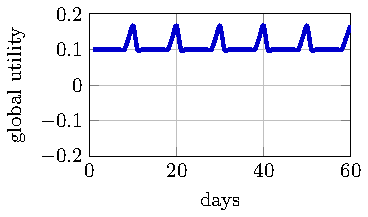
\includegraphics[width=0.3\linewidth]{008_team_6_agent_design/A/SOMAS_A1_utility.pdf} &   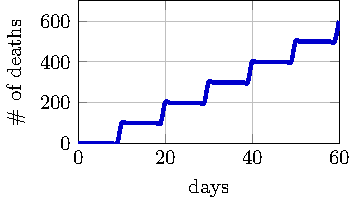
\includegraphics[width=0.3\linewidth]{008_team_6_agent_design/A/SOMAS_A1_deaths.pdf} \\[0pt]
    (a) A1: utility over time & (b) A1: deaths over time \\[8pt]
     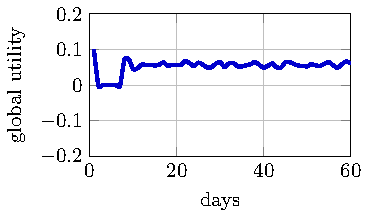
\includegraphics[width=0.3\linewidth]{008_team_6_agent_design/A/SOMAS_A2_utility.pdf} &   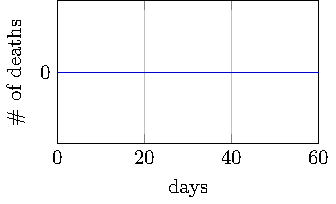
\includegraphics[width=0.3\linewidth]{008_team_6_agent_design/A/SOMAS_A2_deaths.pdf} \\[0pt]
    (c) A2: utility over time & (d) A2: deaths over time
    \\[8pt]
     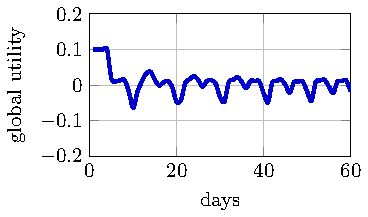
\includegraphics[width=0.3\linewidth]{008_team_6_agent_design/A/SOMAS_A3_utility.pdf} &   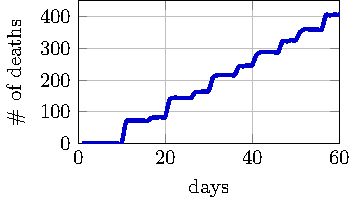
\includegraphics[width=0.3\linewidth]{008_team_6_agent_design/A/SOMAS_A3_deaths.pdf} \\[0pt]
    (e) A3: utility over time & (f) A3: deaths over time
    \\[8pt]
     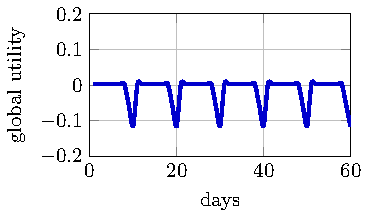
\includegraphics[width=0.3\linewidth]{008_team_6_agent_design/A/SOMAS_A4_utility.pdf} &   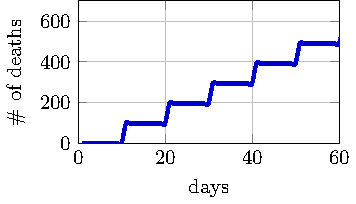
\includegraphics[width=0.3\linewidth]{008_team_6_agent_design/A/SOMAS_A4_deaths.pdf} \\[0pt]
    (g) A4: utility over time & (h) A4: deaths over time
    \end{tabular}
    \caption{Simulation results for a group of agents with uniform fixed social motive.}
    \label{fig:res_A}%
\end{figure}



As expected, a system containing purely altruists (\Cref{fig:res_A} (a) and (b)) leads to the inevitable death of its agents, since by acting purely selflessly, these agents never take any resources from the tower.

As all agents die at the same moment and are all replaced by a new group of altruists, we see a clear pattern in the curve describing the number of deaths over time: after 10 days without eating, all of the agents die, leading to a step of 100 deaths. 

This step pattern is coupled with the global utility. Indeed, each 10 days, there arises a spike in global utility. This can easily explained by \eqref{utility_per_agent}, which states that the utility of the each agents will be positive in this case.

Similar to the altruist agents, the narcissists have a large number of deaths among them every 10 days (\Cref{fig:res_A} (h)). This is evidently due to the agents located on the upper floors of the tower taking all of the food, leaving none for the agents below. In comparison to the altruists, a system composed of narcissists will show negative peaks of global utility, as can be seen in \Cref{fig:res_A} (g). This can be explained using the exact opposite reasoning for the altruistic case - agents no longer vie for maximal resources and receive nothing.

As a compromise between these two systems, a system including only selfish agents presents smoother curves (\Cref{fig:res_A} (e) and (f)). These agents take less food than the narcissists, but still take too much to maintain zero deaths in an economy of scarcity.

Finally, the collectivists instantaneously achieve a stable society in which none of the agents die (\Cref{fig:res_A} (d)). This is due to their innate strategy regarding food intake that ensures the optimal distribution and intake of the common pool resources.

We also note a uniformly positive curve for global utility over time that is smoother than for the other social motives (\Cref{fig:res_A} (c)). This clearly reflects the increased social cohesion between the agents in the tower and identifies the almost perfect allocation of resources, leading to no wasted utility.

As a conclusion from these experiments, we can now state that Hypotheses 1 and 2, formulated in \Cref{hypothesis}, hold in this context.

%%%
\subsubsection{Simulation B: Multiple Agent Types Without Behaviour Change}

Having assessed groups of agents of each social motive individually in Section \ref{sec:simA}, we increase the complexity of the system by having agents with different \textit{fixed} social motives in the tower. The inability for these agents to change their social motive with time leads to the simulation results shown in \Cref{fig:res_B}.

\begin{figure}[H]
    \centering
    \begin{tabular}{cc}
    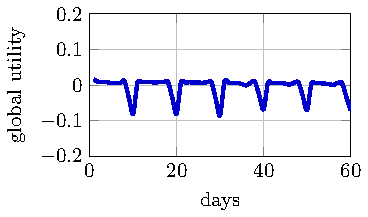
\includegraphics[width=0.3\linewidth]{008_team_6_agent_design/B/B1_utility.pdf} &   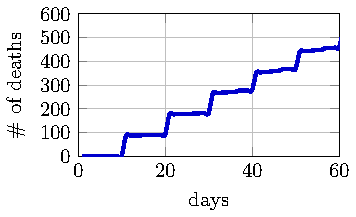
\includegraphics[width=0.3\linewidth]{008_team_6_agent_design/B/B1_deaths.pdf} \\[0pt]
    (a) B1: utility over time & (b) B1: deaths over time \\[8pt]
     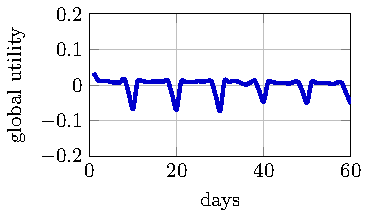
\includegraphics[width=0.3\linewidth]{008_team_6_agent_design/B/B2_utility.pdf} &   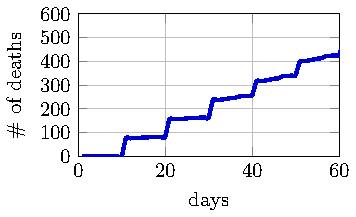
\includegraphics[width=0.3\linewidth]{008_team_6_agent_design/B/B2_deaths.pdf} \\[0pt]
    (c) B2: utility over time & (d) B2: deaths over time
    \\[8pt]
    \end{tabular}
    \caption{Simulation results for a group of agents with different fixed social motives.}
    \label{fig:res_B}%
\end{figure}

The first conclusion we can draw from these results is that having a larger proportion of collectivists helps the system to perform better in terms of utility and number of deaths. Through comparing B1 to B2, we see that the system comprising a larger amount of collectivists (B2) outperforms the system with a comparatively smaller amount of collectivists (B1). This is to be expected, as the more collectivist agents there are, the more similar to \Cref{fig:res_A} (c-d) the system will be.

A second behaviour illustrated by this simulation is that the action of introducing treaties (\Cref{proposing_treaties}) is not always relevant. The collectivist agents accept the collectivist and selfish treaty (the collectivist one being more restrictive), but the selfish agents \textit{only} accept the selfish treaty.\footnote{The other types of agents, altruist and narcissist, do not play a role in this analysis. The altruists accept the two treaties and eat nothing, and the narcissist, being even more difficult to convince, will reject the two treaties.} This way, the two agent types are following their natural strategy concerning food intake (\Cref{food_consumption}). Knowing this, the system shows similar results with and without treaties, hence we only show the results where communication is allowed.

%%%
\subsubsection{Simulation C: Multiple Agent Types With Behaviour Change}\label{simulation_C}

This set of simulations builds on top of the framework set by (B), instead investigating the terminal behaviour of a system comprising different distributions of \textit{fluid} social motives. We provide the agents with a non-zero behavioural swing to investigate the changes in distribution, global deaths and utility over 60 iterations. Moreover, we utilise different levels of communication and treaties to contrast the results using the treaties introduced in \Cref{proposing_treaties} (\Cref{fig:res_C} (a-c)). We simulate the system under two other configurations: without considering any form of communication (\Cref{fig:res_C} (d-f)), and by using a different, more restrictive treaty (\Cref{fig:res_C} (g-i)).

This treaty restricts the amount of food its members can take when their health drops below the \textit{weakLevel}:

If \texttt{currentHP} $<$ \texttt{WeakLevel}, take $\leq$ 2 food.\footnote{To implement this treaty, we create a new treaty type, in addition to the existing set \ToDo{cite corresponding section}. We cite the need for this treaty as it not in general being possible to formulate a request to \texttt{take} a maximum amount with a corresponding \texttt{LeaveAmountFood} or \texttt{LeavePercentFood} treaty. The special case ``take 0'' food can be expressed as ``leave 100\% of the food'', but there is in general no such equivalence that holds across the whole tower.}


\begin{figure}[htb]
    \centering
    \begin{tabular}{ccc}
    % 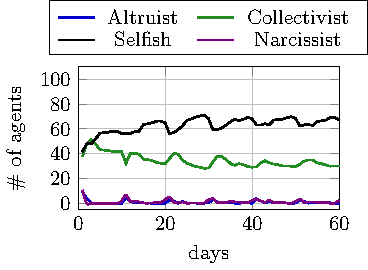
\includegraphics[width=0.3\linewidth]{C/C1_SM.pdf} &   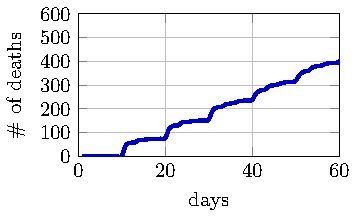
\includegraphics[width=0.3\linewidth]{C/C1_deaths.pdf} &
    % 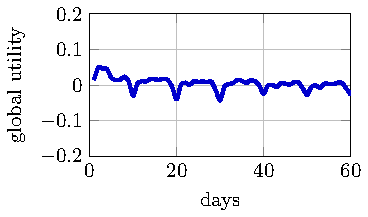
\includegraphics[width=0.3\linewidth]{C/C1_utility.pdf}\\[0pt]
    % (a) C1: social motives & (b) C1: deaths over time & (c) C1: utility over time \\[8pt]
    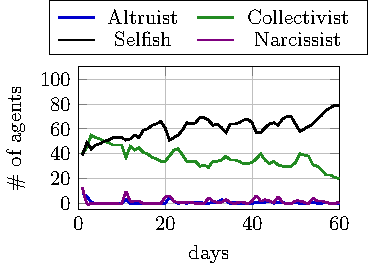
\includegraphics[width=0.3\linewidth]{008_team_6_agent_design/C/C2_SM.pdf} &   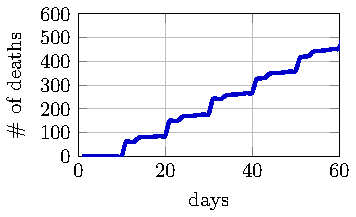
\includegraphics[width=0.3\linewidth]{008_team_6_agent_design/C/C2_deaths.pdf} &
    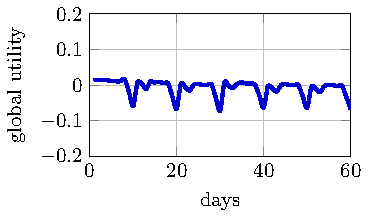
\includegraphics[width=0.3\linewidth]{008_team_6_agent_design/C/C2_utility.pdf}\\[0pt]
    (a) C1: social motives & (b) C1: deaths over time & (c) C1: utility over time \\[8pt]
    % 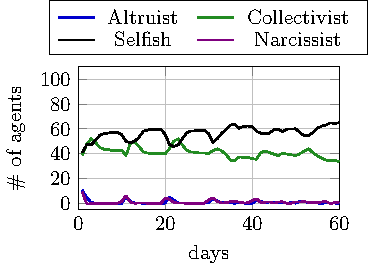
\includegraphics[width=0.3\linewidth]{C/C3_SM.pdf} &   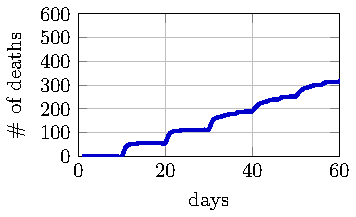
\includegraphics[width=0.3\linewidth]{C/C3_deaths.pdf} &
    % 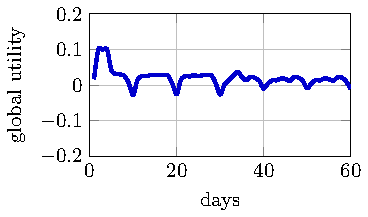
\includegraphics[width=0.3\linewidth]{C/C3_utility.pdf}\\[0pt]
    % (g) C3: social motives & (h) C3: deaths over time & (i) C3: utility over time \\[8pt]
    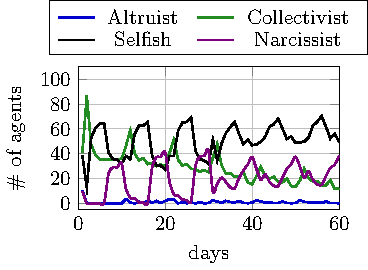
\includegraphics[width=0.3\linewidth]{008_team_6_agent_design/C/C4_SM.pdf} &   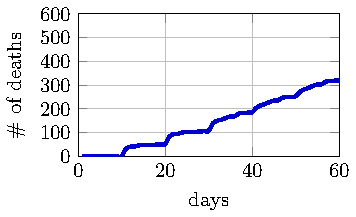
\includegraphics[width=0.3\linewidth]{008_team_6_agent_design/C/C4_deaths.pdf} &
    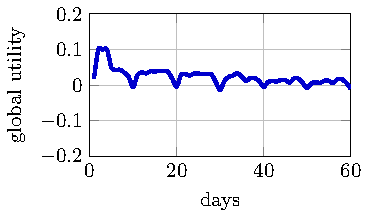
\includegraphics[width=0.3\linewidth]{008_team_6_agent_design/C/C4_utility.pdf}\\[0pt]
    (d) C2: social motives & (e) C2: deaths over time & (f) C2: utility over time \\[8pt]
    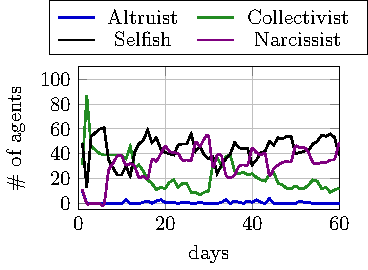
\includegraphics[width=0.3\linewidth]{008_team_6_agent_design/C/C5_SM.pdf} &   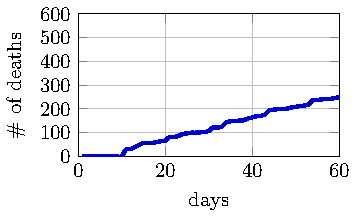
\includegraphics[width=0.3\linewidth]{008_team_6_agent_design/C/C5_deaths.pdf} &
    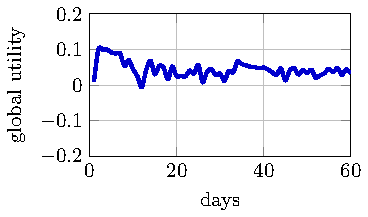
\includegraphics[width=0.3\linewidth]{008_team_6_agent_design/C/C5_utility.pdf}\\[0pt]
    (g) C3: social motives & (h) C3: deaths over time & (i) C3: utility over time \\[8pt]
    \end{tabular}
    \caption{Simulation results for case C. C1 and C3 include communication, but C2 does not. C3 includes a more restrictive treaty.}
    \label{fig:res_C}%
\end{figure}

% C2 was renamed C1, C4 renamed C2. We dropped the initial  


% C4 = less stable than C2
% C4 has death increase after day 30 = reshuffle
% Narcissist can survive with no comms, acting individually - get killed with partial comms in C2 (unlike D with forced comms, where they must act collectivist)


The overarching comment to draw from this set of results is the impact of specific treaties on the global utility. By comparing the results C1 and C2, the system using the `classical' collectivist treaty (C1) (see \Cref{proposing_treaties}) yields a lower performance than the system without treaties (C2): the number of deaths is lower in C2, and its global utility is higher.

To explain these rather counter-intuitive results, we offer the following hypothesis. As the agents' health falls, their social motives tend to change toward narcissist. In the case of collectivists having signed a treaty, they will turn selfish. Instead of following the natural decision of this social motive (eat to stay above the healthy level), they have to follow the treaty. The moment their health falls below the \texttt{weakLevel}, the treaty they signed no longer applies and they will follow their natural food intake rule defined in \Cref{food_consumption}:

If the agent's health is less than the \texttt{healthyLevel}, the agent takes enough food to reach the \texttt{healthyLevel}.

However, this leads to a lot of wasted resources at this critical health level. Notably, each food intake greater than 2 will not offer additional utility to agents whose health falls below the \textit{weakLevel}: any food intake greater than or equal to 2 upgrades the agents health to the \textit{weakLevel}. The resources would have been used in a better way if the selfish agents, which initially signed the treaty as collectivists, would have been able to eat once their health had just risen above the \textit{weakLevel}.

This waste of common resources induced by agents following the collectivist treaty is arguably due to a poor treaty design. This experiment clearly shows that treaties might also have negative effect on the global utility, although they were originally thought to improve it.

To contrast this results, we can propose a more effective treaty. As explained above, simulation C3 introduced a treaty that applies when the agents HP is below the \texttt{weakLevel}. As can be seen in \Cref{fig:res_C} (h) and (i), this treaty allows the total amount of death to be lower, and the global utility to be higher. This shows that well designed treaties can have a positive impact on the system. However, the treaty specification is not a trivial and straight-forward task, that can even be counter-intuitive.

% ------------------

We also allude to the sense of stability that may be offered with the inclusion of treaties. Through juxtaposing C1 (treaties active) with C2 (treaties absent), we see that C2 is in general oscillatory; selfish and narcissistic agents are distributed inversely whilst supporting a low distribution of collectivist agents (10-20\%) throughout the entire simulation. This is in contrast with C1, where the simulation instead stabilises to a relatively continuous distribution of selfish and collectivist agents before bifurcating in the final 10 turns of the simulation.

The presence of ineffective treaties, similar to D1 can be seen to eradicate the population of narcissistic agents, as illustrated by their general absence ($<$5\%) throughout both simulations. We offer that this is due to a sense of individuality that the narcissists exhibit when unconstrained by treaties, allowing for purely self-interested behaviour that can outperform the more `collectivistic' natures of the collectivist and selfish agents, but ultimately lead to self-destruction.

When utilising communication however, there are more grounds for opinion formation, meaning that narcissistic agents will quickly fall into poor favour with the other agents, leading to less social cohesion. This is supported both with D2, where the narcissistic agents are able to integrate with society so long as they always engage in the relevant treaties, and C3, where the introduction of a harsher treaty yields the same terminal results.

The possible stabilising nature of treaties can also be seen from the immunity to the ``death period'' (the number of days an agent is able to survive in the critical region before dying) in C1 and C3. Whilst C2 displays clear oscillatory behaviour with a period of 10 days (occurring at the ``death period''), this susceptibility to such a period is no longer present in graphs C1 and C3, illustrating that treaties offer a sense of immunity. This means that agents will in general not fall within the \texttt{criticalLevel} upon injection and be able to remain in the tower for longer.

This set of experiments supports Hypothesis 5, showing that through careful treaty selection, global utility can be increased in comparison to the case where treaties are disabled (C3 resp. C2). However, the exact selection of these effective treaties is not a trivial task.

% Generally, when unconstrained by treaties and without consistent communication, C4 further suggests that the tendency of all agents is to become more narcissistic, as illustrated by the continual decline of collectivist agents giving rise to an increase in selfish and narcissistic agents. We again contrast with C2 to see that there is no general tendency to move to one end of the spectrum. This stability is again supported through analysis of the reshuffle period: C4 has a clear change in distribution when the reshuffle point at day 30 is reach, whereas the distribution in C2 remains close to constant throughout.

% We also make note of the change in death rate from C4, where at the reshuffle period of 30 days, there is a significant increase in deaths, resulting in approximately 100 more than expected. This can be attributed to the relocation of narcissistic agents to higher floors, giving greater access to food and allowing for more self-interested organisation.

% Experiments C1 and C3 mirror the experiments performed in C2 and C4, observing the response of fluid social motives to an economy of scarcity when communications are both active and inactive. The difference between these two sets stems from the stubbornness of the agents, with C2/4 using a value of 0.2 (very susceptible to change) and C1/3 using a value of 0.8 (very resistant to change).

% This setup produces comparably less emergent behaviours, as agents are effectively restricted between the social motives of collectivist and selfish (in general maintaining the initialisation of a 1:4:4:1 ratio of agents). The magnitude of behavioural update is generally too insignificant to disrupt the equilibrium of collectivists to selfish agents through the introduction of a narcissist, say, so the system effectively stabilises from initialisation.


%%%
\subsubsection{Simulation D: Destabilisation of a Collectivist System}

In these experiments, we initialise the tower's population with collectivist agents only however, unlike with Simulation A (\Cref{sec:simA}), these agents have the possibility to change their social motive over time. 

The goal of these experiments is to evaluate if a society comprised solely of collectivists is able to remain stable over time, noting that if this is achievable, we expect to see similar results to the ones presented in \Cref{fig:res_A} (c) and (d). In addition, we investigate the effect of treaties on such a system. The simulation results are shown in \Cref{fig:res_D}.

\begin{figure}[H]
    \centering
    \begin{tabular}{ccc}
    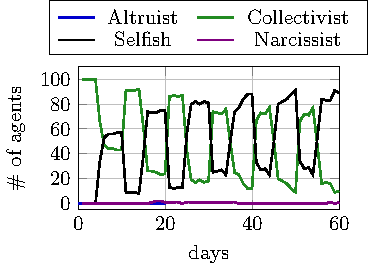
\includegraphics[width=0.3\linewidth]{008_team_6_agent_design/D/D1_SM.pdf} &   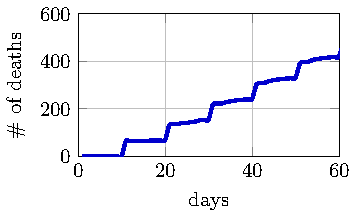
\includegraphics[width=0.3\linewidth]{008_team_6_agent_design/D/D1_deaths.pdf} &
    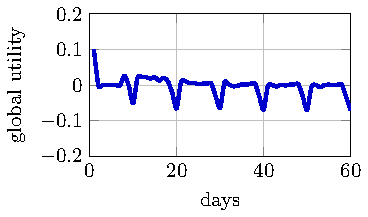
\includegraphics[width=0.3\linewidth]{008_team_6_agent_design/D/D1_utility.pdf}\\[0pt]
    (a) D1: social motives & (b) D1: deaths over time & (c) D1: utility over time \\[8pt]
    %      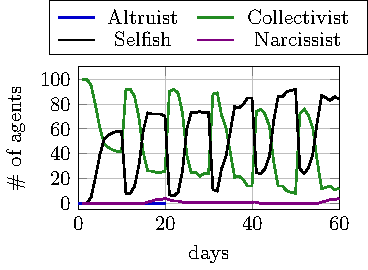
\includegraphics[width=0.3\linewidth]{D/D2_SM.pdf} &   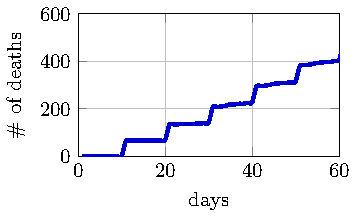
\includegraphics[width=0.3\linewidth]{D/D2_deaths.pdf} &
    % 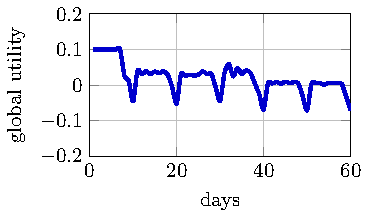
\includegraphics[width=0.3\linewidth]{D/D2_utility.pdf}\\[0pt]
    % (d) D2: social motives & (e) D2: deaths over time & (f) D2: utility over time \\[8pt]
    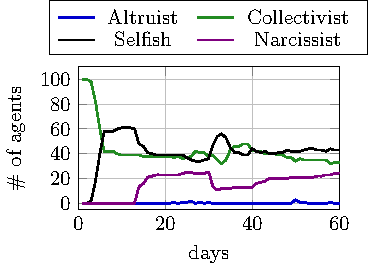
\includegraphics[width=0.3\linewidth]{008_team_6_agent_design/D/D3_SM.pdf} &   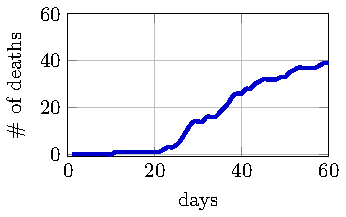
\includegraphics[width=0.3\linewidth]{008_team_6_agent_design/D/D3_deaths.pdf} &
    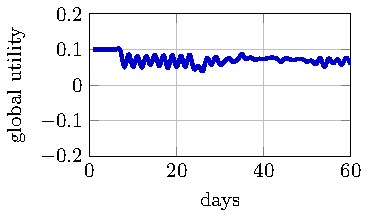
\includegraphics[width=0.3\linewidth]{008_team_6_agent_design/D/D3_utility.pdf}\\[0pt]
    (d) D2: social motives & (e) D2: deaths over time & (f) D2: utility over time \\[8pt]
    \end{tabular}
    \caption{Simulation results different treaties acceptances.}
    \label{fig:res_D}%
\end{figure}

The analysis of experiment D1 can be done as follows: during the first days in the tower, the agents will agree on collectivist treaties as introduced in \Cref{proposing_treaties}. As time progresses and their health decreases, some agents change their social motive from collectivist to selfish (\Cref{fig:res_D} (a)). However, once their health falls below the \textit{weakLevel}, the treaties the agents signed whilst being collectivist no longer apply. This is because, as explained in \Cref{proposing_treaties}, the treaties proposed by collectivists only hold under the condition \textit{currentHP} $>$ \textit{WeakLevel}. Therefore, the selfish agents, now unconstrained, consume more food than what a collectivist agent normally would. This wastes utility, ultimately leading to a large number of deaths at the end of day 10 (\Cref{fig:res_D} (b)). This result is similar to the one discussed in \Cref{simulation_C}.

The waste of common pool resources can also be visualised in \Cref{fig:res_D} (c), where the global utility becomes negative on day 10 (how long agents can survive without eating).

After 10 days, dead agents are replaced by a new group of collectivist agents, leading to a peak in \Cref{fig:res_D} (a). During days 11 to 20, no deaths are seen (\Cref{fig:res_D} (d)), as all selfish agents are still following the treaty they signed when collectivist. Note that the new agents introduced on day 11 sign the collectivist treaties and will not eat any food if their health is above the \textit{weakLevel}, even if they become selfish. On day 20, we note a new peak in the number of deaths, and this process repeats itself. This results in oscillatory behaviour between two quasi-stable states, with convergence to both a high concentration of collectivists and selfish agents in inverse proportions. We hence deem this experiment as 2-phase polystable \cite{ashby2015design}.

% In addition to the treaty used in experiment D1, the agents have the ability to propose and accept the following treaty in experiment D3 \ToDo{rename D3 to D2 and drop the current D2 experiment which is redundant}: 


To avoid selfish agents from wasting common pool resources when their health drops below the \textit{weakLevel}, the agents sign another, more restrictive treaty during the first days of the simulation as in D3 (\Cref{simulation_C}). We note two interesting results when using this additional treaty.

Initially, even the collectivist agents refuse this new treaty. Without knowledge of the motivation of the agents above, each agent utilises forecasting (\Cref{sec:forecasting}) based on their memory of the food they have previously received to evaluate the utility of the expectation of food to be received in the future. We propose that this initial treaty refusal is due to the fact that the computed utility of signing the treaty is smaller than the computed utility based on their estimation of the available food they would get without signing the treaty. We note, however, that the memory of the agents is not yet extensive and that the only exposure to the platform thus far is a cornucopia of resources that nobody touches. 

% The agents are not clever enough to \textit{predict} that this platform will be less full when the agents living above them will have an HP dropping under the weak level. Therefore, they make a rational choice based on their memory and (incomplete \ToDo{find a better word?}) forecasting: they refuse the treaty because they rate the utility of the possible less than 2 food ration proposed by the treaty to be smaller than the amount of food they are forecasting.  

To further investigate the importance of treaties, we override the initial decision of the collectivist agents to accept the treaty. This additional personal risk results in an overall benefit for the society, as seen in \Cref{fig:res_D}. Quantitatively, the number of deaths over time in this scenario is approximately 10 times smaller than in experiment D1 (\Cref{fig:res_D} (e)), accompanied by a uniformly positive utility over time (\Cref{fig:res_D} (f)). In addition, the initial acceptance of this new treaty also allows for the emergence of a stable distribution of social motives across the tower (\Cref{fig:res_D} (d)).

Despite the presence of selfish (and even narcissistic) agents in the tower, they all follow the rule dictated by the treaties they signed whilst being collectivist\footnote{The simulation enforces \textit{honest} agents that do not have the ability to break a treaty before the expiration date. We leave the concept of deception for future work.}. An issue with this configuration is that the exact day when the agents are eating is not synchronised, leading to the selfish and narcissistic agents eating two food as soon as their health falls below the \textit{weakLevel}. We hence conclude that not waiting in the critical zone as collectivists do leads to a non-zero number of deaths.

In addition, we can also see the effect of the reshuffle period on the social motives distribution in \Cref{fig:res_D} (d). The reshuffle period is 30 days in this case and we see that the reorganisation of the tower leads to some of the narcissistic agents updating their social motive to revert to selfish.

The main observation to draw from these results is in the terminal behaviour and the capability to reach stability, with the distribution of all agent types tending to a continuous value (approximately 40\% collectivist, 40\% selfish and 20\% narcissist). We propose that it is this enforcement of treaties that allows for otherwise self-interested agents to act selflessly, instead acting towards a common goal of collectivism. This re-stabilisation of the initially homogeneous collectivist society through treaties is so powerful that it can support a substantial proportion of narcissistic agents, who have in previous experiments (A4, C4) been sufficient for disrupting the stability of a system even in low concentrations. We thus conclude that the inclusion of localised governance allows agents to transcend the limitations of impulsive behaviours due to pre-defined social behaviours and self-organise to maintain a stable system that supports all behavioural types.

These results support the emergence of long-term stability, as stated in Hypothesis 3, when using treaties. D1 shows a regular oscillatory behaviour whereas D2 shows a very constant distribution of the social motives.

Finally, these simulations also clearly show that it is not explicitly necessary to inject external non-collectivist agents in the system to destabilize an otherwise purely collectivist system. Collectivists themselves, if they have the ability to change their social motives, will destroy an originally pure collectivist society. This result is even more drastic than Hypothesis 4.


%%%
\subsubsection{Simulation E: Genetic Replacement of Agents}

This set of simulations aims to assess the effect of \textit{genetic replacement} \cite{vacher1998genetic} \cite{froese2003steps} in creating a system that converges to a static distribution of social motives. For this experiment, we re-inject agents into the tower with a probability equal to that of the current distribution; given a tower consisting of 50\% collectivists and 50\% selfish agents, say, there will be an equiprobable chance of the next agent added to the tower being either of these types.

\begin{figure}[htb]
    \centering
    \begin{tabular}{ccc}
    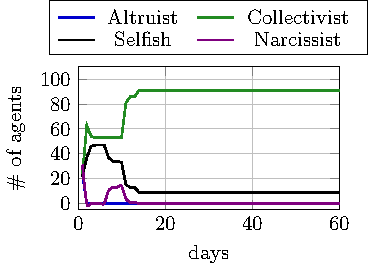
\includegraphics[width=0.3\linewidth]{008_team_6_agent_design/E/E1_SM.pdf} &   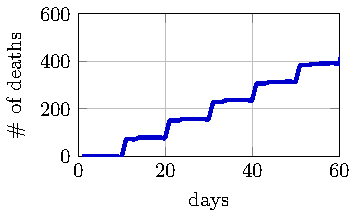
\includegraphics[width=0.3\linewidth]{008_team_6_agent_design/E/E1_deaths.pdf} &
    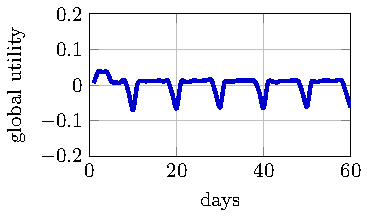
\includegraphics[width=0.3\linewidth]{008_team_6_agent_design/E/E1_utility.pdf}\\[0pt]
    (a) E1: social motives & (b) E1: deaths over time & (c) E1: utility over time \\[8pt]
         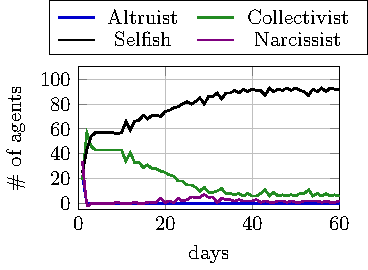
\includegraphics[width=0.3\linewidth]{008_team_6_agent_design/E/E2_SM.pdf} &   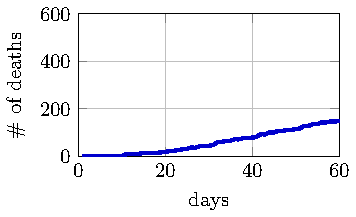
\includegraphics[width=0.3\linewidth]{008_team_6_agent_design/E/E2_deaths.pdf} &
    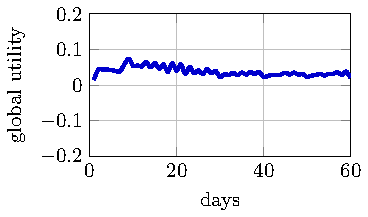
\includegraphics[width=0.3\linewidth]{008_team_6_agent_design/E/E2_utility.pdf}\\[0pt]
    (d) E2: social motives & (e) E2: deaths over time & (f) E2: utility over time 
    \end{tabular}
    \caption{Simulation results with genetic replacement of the agents.}
    \label{fig:res_E}%
\end{figure}

% Genetic replacement is a way to replace the dead agents using the current distribution of the social motives across the tower. If a dead agent needs to be replaced and that the proportion of collectivist in the tower is 70\%, there is a probability of 70\% that the new injected agent will be collectivist.

% The main purpose of this experiment is to see if the system converges to some equilibrium with respect to social motives distribution, and if so, to see if we reach a system where global utility is maximized. All simulation start with an even distribution regarding the agents social motives (25\% of each social motive).

Starting with an equal distribution of all agent types (25\% of each social motive), we not only investigate the terminal behaviours of the system regarding stability, but whether or not this system can maximise its global utility. As described in \Cref{simulation_summary}, E1 and E2 differ by the quantity of resources available in the common pool, with E1 representing a strict economy of scarcity and E2 an economy of abundance. We first present and discuss the results achieved in an economy of scarcity (setup E1, \Cref{fig:res_E} (a), (b), and (c)).

It is clear from \Cref{fig:res_E} (a) that the system E1 achieves a stable distribution of the social motives over time, with a ratio of 90\% Collectivists to 10\% Selfish agents. This distribution leads to fewer deaths than in a purely selfish society (see \Cref{fig:res_A} (f)), but significantly more deaths than in a purely collectivist society (see \Cref{fig:res_A} (d)). The global utility shows clear peaks at the end of every critical period of 10 days (\Cref{fig:res_E} (b)).

In a scenario where there is enough food to not only satisfice, but also satisfy each agent on every given day (thus removing an economy of scarcity), the dominant social motive is selfish. This emergence can be attributed to the valuation assigned to treaties: if there is a continual supply of food, treaties offer very little utility to the selfish agents and are hence rejected. Unlike in D1, where the oscillatory behaviour was a product of the selfish agents' inability to survive, we now impose a system where selfish behaviour \textit{can} be supported, due to the higher availability of food. Furthermore, the low number of deaths (\Cref{fig:res_E} (e)) and the relatively high utility (\Cref{fig:res_E} (f)) are not due to the social motive distribution, but instead the amount of food on the platform, which is larger than usual.

To answer the statement introduced in Hypothesis 6, we see with these experiments that convergence of the system strongly depends on the quantity of resources available in the common pool.

 
%%%%%%%%%%
%%%%%%%%%%% CONCLUSION AND FUTURE WORK
%%%%%%%%%%%%%%%%%%%%%%%%%%%%%%%%%%%%%%%
\section{Conclusion and Future Work}\label{conclusion_future_work}

\subsection{Conclusion}

In conclusion, we utilise the codification of social motives to offer insight into the general tendency of behavioural changes in an economy of scarcity, as well as the efficiency of treaties in stabilising a population comprising various different social motives. 

Irrespective of initialisation, the natural tendency of agents in an economy of scarcity is to make a transition towards the narcissistic end of the spectrum (B-D), leading to a higher overall distribution of selfish agents. Genetic replacement serves as a means of avoiding this behaviour, showing a clear stabilisation to an almost uniformly collectivist population (E1), but is contrasted by a drastic tendency towards selfishness when more resources are made available to the set of agents (E2).

Treaties serve as a stabilising self-organising mechanism in this set of experiments, with appropriately constrictive treaties (C3, D2) even allowing for the stable integration of narcissists into the population, despite their natural tendency to destabilise a system (A4, C2). Treaties may also change a polystable system into a purely stable system, when sufficiently strong as to enforce a collectivist mindset (D1, D2), converting an otherwise oscillatory distribution of social motives into a static distribution.

We hence assert that treaties are a sufficiently powerful self-organising mechanism to mitigate the collective action problem that this platform imposes, as they can be seen to increase global utility (C3, D2) and stabilise global deaths. This affirms that, whilst self-governing institutions cannot be formed, it is through honest following of treaties that an unstable population can be controlled to produce a uniform distribution of social motives.
 
\subsection{Future Work}
Our future work would focus around adapting the ways in which we model the agents' changes in social motives. One such way is to make agents tend towards altruism, rather than narcissism, when faced with adversarial conditions. This could be interpreted as an understanding of the agent's environment and the long-term improvement of the individual utility through a short-term sacrifice, in the sense that it is expected that other agents would act similarly, thus bringing the system back to an equilibrium. This would be done by changing the weights used in the social motive update function.

Furthermore, we might imagine a randomly distributed assignment of these weights across different agents. This would illustrate how different agents might react differently to their condition, from which the concept of agent personality could be derived. For example, some agents may encounter a comfortable situation (high HP, high floor) and decide to take advantage of it and act selfishly, while another agent may encounter the same situation and take the opportunity to make a positive impact for their fellow agents below by acting altruistically.

Also, one might make the assumption that the agent's true personality comes forth under beneficial circumstances, whereas a harsh environment is likely to cause the agent to act differently. If the agent's genotype can be defined as the agent's true personality, then the agent's phenotype, i.e., their resulting behaviour, can be modelled by interpolating between this genotype and the social motives based purely on environmental factors. Combining this concept with the random weights assignment may allow for the modelling of both the agent's genotype and their reaction to environmental variables based on their personality.

Finally, we would analyse the effects of a larger number of treaties on the global utility. As shown in this work, the choice of treaties leading to an increase in the global utility is not straightforward. As treaties are expressed in a generic way, it is possible to tune a large number of parameters to find optimal treaties in a given scenario.


